\documentclass[11pt,letterpaper]{article}
%\usepackage[round]{natbib}
\usepackage{emnlp2016}
\usepackage{amsmath}
\usepackage{paralist}
\usepackage{subfig}
\usepackage{times}
\usepackage{latexsym}
\usepackage{graphicx}
\usepackage{url}
\usepackage{pgfplotstable}
\usepackage{titlesec}
%\usepackage{hyperref}
\usepackage{color}
\usepackage{lipsum,adjustbox}
\usepackage[font={small}]{caption}

\def\emnlppaperid{***}
\setlength{\belowcaptionskip}{-10pt}

\makeatletter

%\titlespacing*{\section}
%{0pt}{1ex plus 1ex minus 1ex}{1ex plus .2ex}
%\titlespacing*{\subsection}
%              {0pt}{1ex plus 1ex minus 1ex}{1ex plus .2ex}

\titlespacing{\section}{2pt}{*0}{*0}
\titlespacing{\subsection}{2pt}{*0}{*0}
\titlespacing{\subsubsection}{2pt}{*0}{*0}
\titlespacing{\paragraph}{1pt}{*0}{3pt}

              

\makeatother



\listfiles

\newcommand{\com}[1]{}
\newcommand{\secref}[1]{\S\ref{#1}}
\newcommand{\figref}[1]{Figure~\ref{#1}}
\newcommand{\tabref}[1]{Table~\ref{#1}}
\newcommand{\XXX}[1]{{\color{red}XXX #1}} % a general todo or comment
%\newcommand{\XXX}[1]{}
%\newcommand{\oa}[1]{\footnote{\color{red}OA: #1}}
\newcommand{\oa}[1]{}
\newcommand{\bh}[1]{\footnote{\color{blue}BH: #1}}
%\newcommand{\bh}[1]{}

\def\perscite#1{\newcite{#1}}
\def\parcite#1{\cite{#1}}
\def\inparcite#1{\cite{#1}}

\def\equo#1{``{#1}''}  % curly quotes

\newcommand\BibTeX{B{\sc ib}\TeX}

\listfiles

% better maths typography
\def\setsize#1{\lvert #1 \rvert}
\def\func#1{\text{\it #1}}  % much better kerning within function names
\def\HUME{\func{HUME}}
\def\Adequate{\func{Adequate}}
\def\Green{\func{Green}}
\def\Orange{\func{Orange}}
\def\Units{\func{Units}}


\title{HUME: Human UCCA-Based Evaluation of Machine Translation}

\author{Author 1\\
	    XYZ Company\\
	    111 Anywhere Street\\
	    Mytown, NY 10000, USA\\
	    {\tt author1@xyz.org}
	  \And
	Author 2\\
  	ABC University\\
  	900 Main Street\\
  	Ourcity, PQ, Canada A1A 1T2\\
  {\tt author2@abc.ca}}

\date{}

\begin{document}

\maketitle

\begin{abstract}
  
%  Recent interest in semantics-aware MT systems underscores the importance of
%  semantic evaluation for Machine Translation (MT) systems. 
%  A semantic measure, sensitive to possible semantic discrepancies
%  between the translation output and the source, is likely to support the construction
%  and tuning of semantics-based MT, much in the same way that string-based measures,
%  such as BLEU, enabled progress in shallower MT.
%  We present a novel human semantic evaluation measure for MT, Human
%  UCCA-based MT Evaluation (HUME), building on the UCCA semantic representation scheme.
%  Making progress over previous work, the proposed measure takes into account
%  a wider range of semantic phenomena and does not rely on semantic annotation
%  of the MT output itself, whose interpretation is often unclear.
%  We experiment with four language pairs, demonstrating HUME's broad applicability,
%  as well as its reliability, reflected in its inter-annotator agreement rates.

Human evaluation of machine translation normally uses sentence-level measures such as relative ranking or adequacy scales. However these provide no insight into possible errors,
and do not scale well with sentence length.
We argue for a semantics-based evaluation, which captures what meaning components
are retained in the MT output, providing a more fine-grained analysis of
translation quality, and enables the construction and tuning of semantics-based MT. 
We present a novel human semantic evaluation measure, Human
UCCA-based MT Evaluation (HUME), building on the UCCA semantic representation scheme.
%Making progress over previous work, the proposed measure takes into account
HUME covers
a wider range of semantic phenomena than previous methods and does not rely on semantic annotation
of the potentially garbled MT output. 
%itself, whose interpretation is often unclear.
We experiment with four language pairs, demonstrating HUME's broad applicability,
and report good
%as well as its reliability, reflected in its 
inter-annotator agreement rates and 
 correlation with human adequacy scores.


%Human evaluation of machine translation is a cognitively difficult task and when
%annotators rate or rank complete sentences, we see low levels of agreement especially
%for longer sentences.  
%In order to extract more reliable annotations, previous research broke down evaluation into smaller 
%components by asking humans to annotate semantic roles on the source and translation, and then to align them. 
%In order to extract more reliable annotations, previous research broke down
%evaluation into smaller components in various ways. 
%We propose a new evaluation method
%HUME
%which is based on semantic annotation called Universal Conceptual Cognitive Annotation (UCCA). UCCA
%is applicable across many languages, it provides a complete structure over sentences, and it is 
%grounded in the words in the sentence. 
%We apply UCCA only over the source or reference sentence, and not over the
%possibly garbled translation.
%, 
%and this makes annotation more reliable and also efficient as we can reuse labor
%intensive semantic annotations.
%We show that HUME can be reliably applied to
%four different target languages and that sentence level inter-annotator agreement
%does not decrease over longer sentences. 

\end{abstract}


%%%%%%%%%%%%%%%%%%%%%%%%%%%%%%%%%%%%%%%%%%%%%%%%%%%%%%%%%%%%%%%%%%%%%%%%%%%%%%%%%%%%%%
\section{Introduction}\label{sec:intro}

Human judgement is the cornerstone for estimating the quality of an MT system.
Nevertheless, common measures for human MT evaluation, such as adequacy and fluency judgements
or the relative ranking of possible translations, are problematic in two ways.
First, as the quality of translation is multi-faceted, it is difficult
to quantify the quality of the entire sentence in a single number. This
is indeed reflected in the diminishing inter-annotator agreement (IAA) rates of human ranking measures
with the sentence length \cite{Bojar:2011}.
Second, a sentence-level quality score does not indicate what parts of the sentence
are badly translated, and so cannot inform developers in repairing these errors.

These problems are partially addressed by measures that decompose over parts of the evaluated
translation. For automatic measures,
these are often words or n-grams, for manual measures some structural
information is taken into account \parcite{machacek:bojar:segranks:2015}, or the
annotators are explicitly asked to mark errors, which however suffers from even
lower agreement than ranking \parcite{lommel:etal:mqm-iaa:2014}.
% the following is specific to automatic measures:
%quantifying the overlap of its sub-parts relative a reference translation.
A promising line of research decomposes metrics
over semantically defined units,
quantifying the similarity of the output and the reference in terms of
their verb argument structure; the most notable of these measures is HMEANT
\parcite{lo2011structured}.
%More recent work on MT evaluation proposed measures
%that decompose

% SAVING SPACE:
% \XXX{Do we want to cut the following shorter?}
% However, 
% their focus on verb argument structures misses many semantic phenomena
% (such as inter-clause linkage and nominal argument structures), providing
% only
% a limited perspective on the semantic similarity between the translation and reference.
% Also, assigning semantic structure to an MT output, especially a poor one,
% is difficult and arguably ill-defined.

We propose the HUME metric,
a human evaluation measure that decomposes over the UCCA semantic units.
% of the sentence.
UCCA \parcite{abend2013universal} is an appealing candidate for semantic analysis,
due to its cross-linguistic applicability, support for rapid annotation, and coverage
of many fundamental semantic phenomena, such as verbal, nominal and adjectival
argument structures and their inter-relations.

HUME operates by aggregating human assessments of the translation quality of individual
semantic units in the source sentence. We 
%HUME only requires semantically annotating the source sentence,
are thus avoiding the semantic annotation of machine-generated text,
which is often garbled or semantically unclear.
This also allows the re-use of the source semantic annotation for
measuring the quality of different translations of the same source sentence,
and 
%By basing the measure on a direct comparison
%of the source and translation we avoid the difficulties created by using
avoids relying on possibly suboptimal reference translations.
%albeit at the cost of requiring the
%evaluator to be proficient in both the source and target languages.
%An elaborate comparison of HUME and HMEANT is given in \secref{sec:hmeant_comp}.

%Could reinstate
After a brief review (\secref{sec:background}), we describe HUME in detail
(\secref{sec:hume}).
Our experiments with four language pairs: English to Czech, German, Polish and Romanian (\secref{sec:experiments}) document HUME's inter-annotator agreement and efficiency (time of annotation). We further empirically compare HUME with direct assessment of human adequacy ratings, and conclude by discussing the differences with HMEANT (\secref{sec:hmeant_comp}).

% We conduct experiments with four language pairs: English-German, English-Polish,
% English-Romanian and English-Czech, and report efficiency (time of annotation) and
% inter-annotator agreement scores (\secref{sec:experiments}).
% 
% \XXX{The following should go rather to the conclusion}
% Efficiency results that HUME
% can be annotated in 2--4 minutes, once the UCCA annotation of the source is given,
% which is only about five times slower than MEANT, and hence still practical to
% employ on a moderate scale. HUME's agreement results are on par with those
% of standard sentence-level ranking measures, but unlike them,
% HUME's scores do not decrease with longer sentences.\bh{We may
%   have to focus more on qualitative aspects, if we just try to sell
%   the measure on IAA, then the figures are not stunning. OA: is that OK?}



%%%%%%%%%%%%%%%%%%%%%%%%%%%%%%%%%%%%%%%%%%%%%%%%%%%%%%%%%%%%%%%%%%%%%%%%%%%%%%%%%%%
\section{Background}\label{sec:background}

%While the measure addresses the two major shortcomings 
%detailed above, it is unable to capture semantic differences which do not show up in 
%the verb-argument structure, including several very frequent phenomena, 
%Another shortcoming of MEANT is its reliance on semantically annotating MT output,
%which is often unintelligible. Finally, measures based on a comparison to a


%These difficulties have motivated the definition of a human measure that decomposes over
%the semantic structure of the sentence, rather than its n-grams. The most notable attempt of
%this type is the MEANT measure, and its human variant HMEANT
%\parcite{lo2010evaluating,lo2011structured,Lo2011meant,lo2013meant}, which quantifies the
%similarity between the output translation and a reference translation in terms of the similarity
%between their verbal argument structures
%While the measure addresses the two major shortcomings
%detailed above, it is unable to capture semantic differences which do not show up in
%the verb-argument structure, including several very frequent phenomena, such as
%inter-clause linkage, nominalizations and copula clauses
%(see \secref{sec:hmeant_comp}).
%Another shortcoming of MEANT is its reliance on semantically annotating MT output,
%which is often unintelligible. Finally, measures based on a comparison to a
%reference translation
%are necessarily incomplete, as they compare to a small number of references
%out of the the huge number of possible translations a sentence may have
%\parcite{dreyer2012hyter}.


\paragraph{MT Evaluation.}
%MT evaluation has been traditionally pursued through human-based
%evaluation that quantifies the adequacy of the translation in preserving the meaning 
%of the source sentence, and its fluency as a sentence in the target language
%\parcite{lopez2008statistical}.
Human evaluation is generally done by ranking the outputs of multiple systems
e.g., in the WMT tasks \parcite{bojar2015findings}, or by assigning
adequacy/fluency scores to each translation, a procedure recently improved
by \perscite{graham2015accurate}.
However, while providing the gold standard for MT evaluation, human evaluation
is not a scalable solution.
%and is infeasible where a wide variety of systems or parameter settings are to be evaluated.
% has motivated the construction of cheaper methods that correlate with human
%judgement.

Scalability is addressed by employing automatic and semi-automatic approximations of human
judgements. Commonly, such scores decompose over the sub-parts of
the translation, and quantify how many of these sub-parts appear in a manually created reference translation.
This decomposition allows system developers
to localize the errors.
%, or at least unconfirmed parts within the translation.
The most commonly used measures decompose over n-grams or individual words, e.g., 
BLEU \parcite{Papineni:2002}, NIST \parcite{Doddington:2002} and METEOR
\parcite{Banerjee:2005}.
Another common approach is to determine the similarity between the reference and translation
in terms of string edits \parcite{snover2006study}.
While these measures stimulated much progress in MT research by allowing
the evaluation of massive-scale experiments, the focus on words and n-grams does
not provide a good estimate of semantic correctness, and may favour shallow string-based
MT models.

%These methods are most suitable for evaluating shallow MT approaches and are
%less instructive as to what aspects of the reference's meaning were not preserved
%in the translation output.
%A common approach is to compare the MT output with reference translations,
%created or verified by an expert. Methods often rely on some sort of string matching
%methods, such as overlap of n-grams, as with the BLEU and METEOR measures, or edit
%distance.
%First, they rely on comparison to reference translations, which reflect a small
%number out of the enormous number of ways to translate a sentence and are thus
%inherently incomplete. 

In order to address this shortcoming, more recent work quantified
the similarity of the reference and translation in terms
of their structure. \perscite{liu2005syntactic} took a syntactic approach, 
using dependency grammar, and
\perscite{owczarzak2007evaluating} took a similar approach using lexical-functional grammar structures.
\perscite{gimenez2007linguistic} proposed to combine multiple types of information,
capturing the overlap between the translation and reference in terms of their
semantic (predicate-argument structures), lexical and morphosyntactic features.

Perhaps the most notable attempt at semantic MT evaluation is MEANT and
its human variant HMEANT \parcite{lo2011structured}, which quantifies the similarity between
the reference and translation in terms of the overlap in
their verbal argument structures and associated semantic roles.
We discuss the differences between HMEANT and HUME in \secref{sec:hmeant_comp}.

%\begin{figure}
%
%\begin{tikzpicture}[semithick, x=2.4cm,y=0.8cm, >=latex, baseline=7ex,
%    inner sep=.3ex, outer sep=.7ex, minimum size=1.2ex,->]
%  \node (ROOT) [fill=black, circle] {}
%  child {node {After} edge from parent node[left]  {$L$\hspace{1.5cm}}}
%  child {node (H1)  [fill=black,circle] {}
%    child {node {graduation} edge from parent node[right] {$P$}}
%      %child {node {to Paris} edge from parent node[right] {$A$}}
%      edge from parent node[left] {$H$}
%    }
%    child {node (H2)  [fill=black,circle] {}
%      child {node  {} edge from parent[draw=none]}
%      child {node  {} edge from parent[draw=none]}
%      child {node  (Tom) {Tom} edge from parent node[right] {$A$}}
%      child {node  {moved} edge from parent node[right] {$P$}}
%      child {node  [fill=black,circle] {}
%        child {node  {to} edge from parent node[right] {$R$}}
%        child {node  {NYC} edge from parent node[right] {$C$}}
%        edge from parent node[right] {$A$}}
%      %child {node {to Paris} edge from parent node[right] {$A$}}
%      edge from parent node[left] {$H$}
%    };
%    \draw (H1) -> (Tom) node[midway, right] {$A$ \hspace{0.2cm}};
%  \end{tikzpicture}
%\caption{\label{fig:ucca_example}
%  Sample UCCA annotation of the sentence ``After graduation, Tom moved
%  to NYC''. Leaves correspond to words, whereas nodes correspond to units.
%  Edge labels mark UCCA categories, which are described in the table.}
%%which are largely ignored in this work
%\end{figure}


\begin{figure}
    \begin{center}
    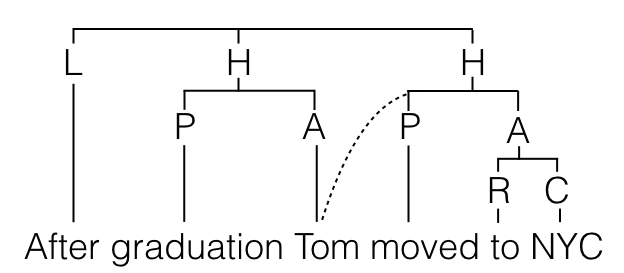
\includegraphics[width=0.35\textwidth]{ucca-tree-v2.png}

{\small
  \begin{tabular}{|l|l|l|l|}
\hline
L & Linker &  A & Participant \\
H & Parallel Scene & R & Relater \\
P & Process & C & Centre \\
\hline
\end{tabular}
}
    \end{center}
\caption{\label{fig:ucca_example_v2}
  Sample UCCA annotation. Leaves correspond to words and nodes to units.
  The dashed edge indicates that ``Tom'' is also a participant in the ``moved to NYC''
  Scene. Edge labels mark UCCA categories.}
%which are largely ignored in this work
\end{figure}

\paragraph{Semantic Representation.}
UCCA (Universal Conceptual Cognitive Annotation, \inparcite{abend2013universal}) is a
cross-linguistically applicable, lightweight
scheme for semantic annotation. Formally, an UCCA structure is a directed acyclic graph (DAG),
whose leaves correspond to the words of the text.
The graph's nodes, called {\sc units}, are either terminals or several elements jointly
viewed as a single entity according to some semantic or cognitive consideration. Edges bear
a category, indicating the role of the sub-unit in the structure the unit
represents.

UCCA's current inventory of distinctions focuses on argument structures
(adjectival, nominal, verbal and others) and relations between them.
The most basic notion is the Scene, which describes a movement, an
action or a state which persists in time. Each Scene contains one main
relation and zero or more participants. For example, the sentence ``After graduation, Tom moved to NYC''
contains two Scenes, whose main relations are ``graduation'' and ``moved''.
The participant ``Tom'' is a part of both Scenes, while ``NYC'' only of the
latter (\figref{fig:ucca_example_v2}). Further categories account for
inter-scene relations and the sub-structures of participants and relations.

% UCCA Motivation
The use of UCCA for semantic MT evaluation measure is motivated by two main reasons. 
First, UCCA's set of categories can
be reliably annotated by non-experts after as little as two hours
of training \parcite{marinotti2014}.
Second, UCCA is cross-linguistically applicable, seeking to
represent what is shared between languages by building on
linguistic typological theory \parcite{Dixon:10a,Dixon:10b,Dixon:12}.
Its cross-linguistic applicability has so far been tested in annotations of
English, French, German and Czech.
%Third, the scheme has been shown to be stable across translations:
%UCCA annotations of translated text usually contain the same set of relations
%\parcite{sulem2015conceptual}, indicating that the scheme reflects
%a common layer of representation that in a correct translation
%is mostly shared between the translation and the source. 

%Verbal argument structures are less stable in this sense, as they
%may be translated or paraphrased to a nominal or adjectival
%argument structure, and is thus less suitable as a basis for a semantic measure.
%E.g., ``after he graduated, Tom moved to NYC'' contains two verbs,
%but is similar in meaning to the one-verbed
%``after graduation, Tom moved to NYC''. 

% While most broad-coverage semantic work focused on shallow semantic structures,
% predominantly argument structures annotated with their semantic roles, much recent
% interest has been devoted to defining more complete semantic representation schemes.
% \oa{should we
% add that it is less cross-linguistically stable? maybe that's an overkill..
%  OB: AMR has been applied to more languages, including Chinese, so I would not
%  dare saying that it is less stable.}

The Abstract Meaning Representation (AMR) \parcite{banarescu2013abstract} project
shares UCCA's motivation for defining a more complete semantic annotation.
However, using AMR is not optimal for defining a decomposition of a sentence into semantic
units as it does not ground its semantic symbols in the text,
and thus does not provide clear decomposition of the sentence into sub-units.
Also, AMR is more fine-grained than UCCA and consequently harder to annotate.
Other approaches represent semantic structures as bi-lexical dependencies
\parcite{sgallhp:1986,hajic2012announcing,oepen2006discriminant},
which are indeed grounded in the text, but are less suitable for MT evaluation
as they require linguistic expertise for their annotation.

%, and so we argue they are less suitable 
%for an interpretable MT evaluation.

%Examples include the tectogrammatical layer  used in the Prague dependency
%treebanks, e.g. the Czech-English one \parcite{}, as well
%as dependencies derived from Minimal Recursion Semantics representations \parcite{}.
%Nevertheless, despite their appeal as deep and intuitive means for semantic representation,

%\perscite{Basile:12} attempted to make some aspects of the semantic annotation more accessible,
%but to our knowledge no results of this brand have been reported.


%%%%%%%%%%%%%%%%%%%%%%%%%%%%%%%%%%%%%%%%%%%%%%%%%%%%%%%%%%%%%%%%%%%%%%%%%%%%%%%%%%%

\vspace{-.1em}
\section{The HUME Measure}\label{sec:hume}
\vspace{-.2em}

\subsection{Annotation Procedure}\label{sec:guidelines}

This section summarises the manual annotation procedure used
to compute the HUME measure. 
We denote the source sentence as $s$ and the translation as $t$. 
The procedure involves two manual steps: (1) UCCA-annotating $s$, 
(2) human judgements as to the translation quality of each semantic unit of $s$ relative to $t$,
where units are defined according to the UCCA annotation.
UCCA annotation is performed once for every source sentence,
irrespective of the number of its translations we wish
to evaluate
%\footnote{Instead of relying on the source,
%the evaluation could be based on the UCCA structure for the \emph{reference}
%translation.
%More details in the discussion in \secref{src-vs-ref}.
% This would allow monolingual annotators to take part in the
% evaluation. On the downside, the translation would have to be aligned to the
% reference and more importantly, we would risk inaccurate judgements due to
% the naturally occurring differences between the source and its reference
% translations.
%}.

\paragraph{UCCA Annotation.}
We begin by creating UCCA annotations for the source sentence, following the
UCCA guidelines\footnote{All UCCA-related resources can be found
  here: \url{http://www.cs.huji.ac.il/~oabend/ucca.html}}.
A UCCA annotation for a sentence $s$ is a labeled DAG $G$, whose leaves
are the words of $s$.
For every node in $G$, we define its {\it yield} to be its leaf descendants.
The semantic units for $s$ according to $G$ are the yields of nodes in $G$. 

%\begin{figure*}[t]
%    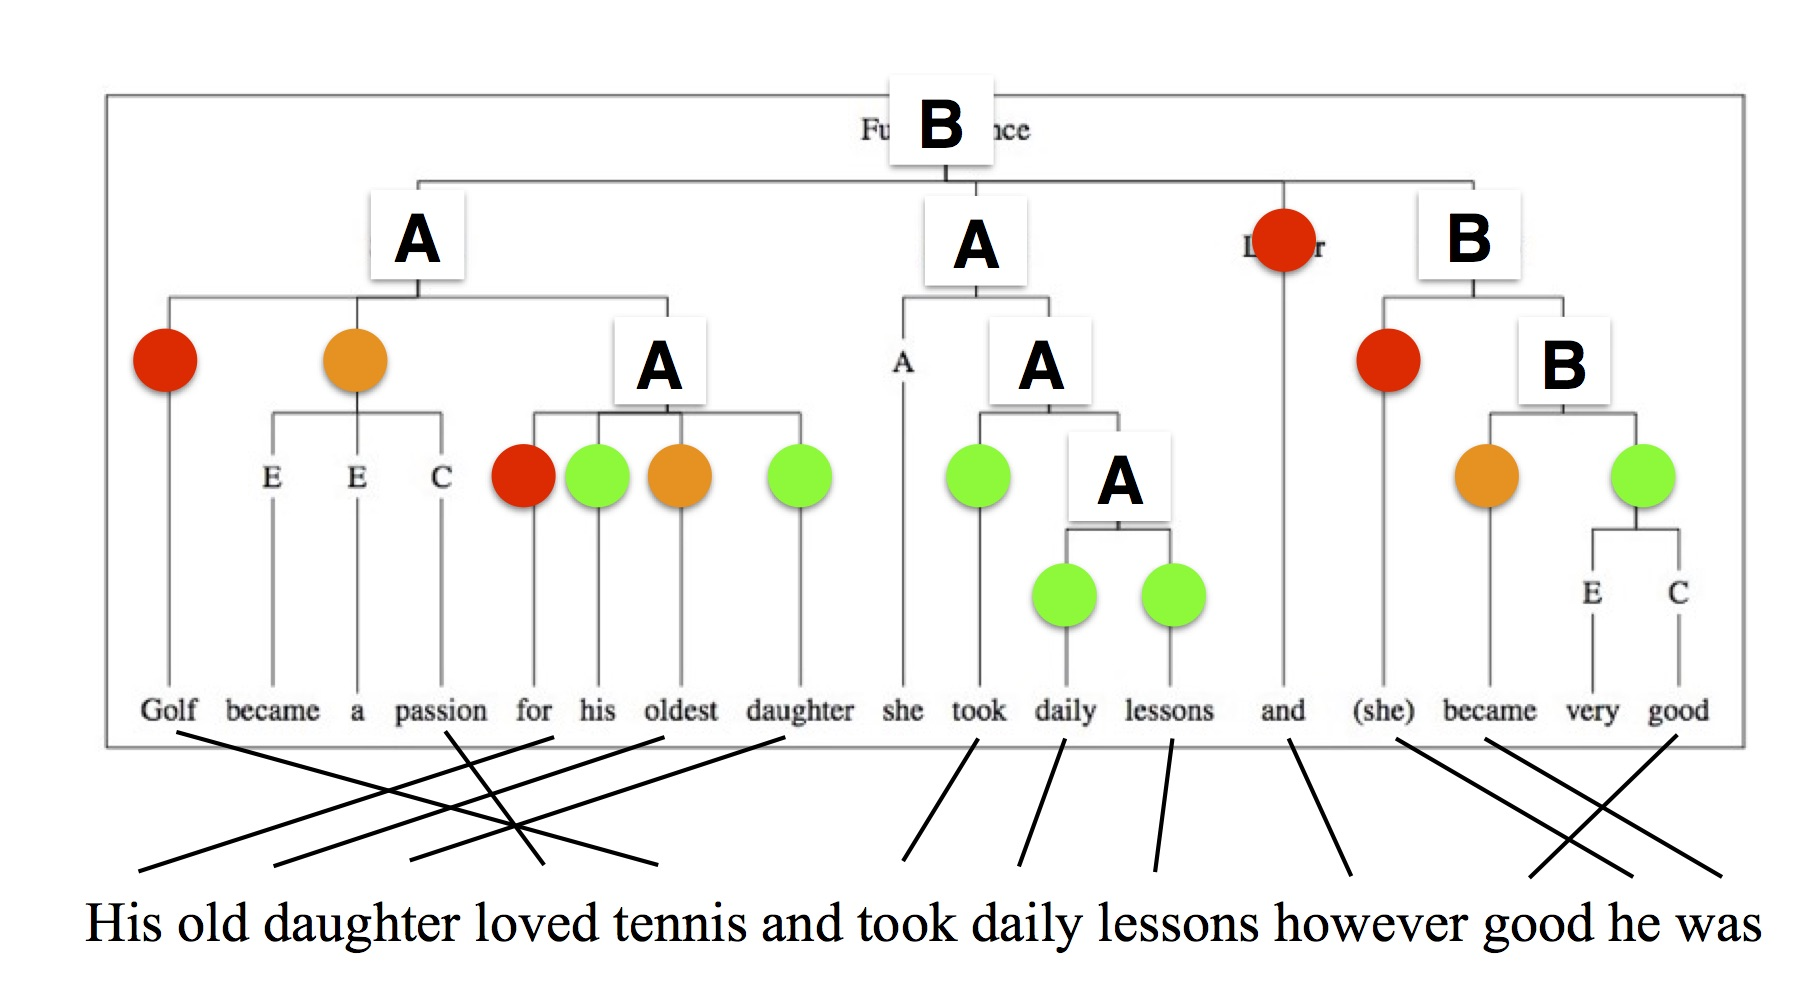
\includegraphics[width=1\textwidth]{ucca-tree-mteval.jpg}
%    \caption{UCCA Tree evaluated in comparison to an aligned ``translation'' (an
%	English paraphrase).}
%    \label{fig:ucca-tree-hume}
%\end{figure*}




%\begin{figure*}
%  \begin{adjustbox}{trim=2.3cm 0 0 0}
%   \begin{tikzpicture}
%     [ level distance=12mm,
%	   level 1/.style={sibling distance=7.5em,level distance=7mm},
%       level 2/.style={sibling distance=5em,level distance=12mm},
%       level 3/.style={sibling distance=5em},
%       level 4/.style={sibling distance=3em}]
%     %[semithick, x=2.4cm,y=0.8cm, >=latex, baseline=7ex,
%     %  inner sep=.3ex, outer sep=.7ex, minimum size=1.2ex,->]
%   \node (ROOT) [label={B}] [fill=blue, circle] {}
%   child {node (H3) [label={A}] [fill=yellow,circle] {}
%     child {node [label={[red]:R}] {Golf} edge from parent node[left] {}}
%     child {node (H1) [label={[orange]30:O}] [fill=orange,circle] {}
%       child {node [label={}] {became} edge from parent node[left]  {}}
%       child {node [label={}] {a} edge from parent node[left]  {}}
%       child {node [label={}] {passion} edge from parent node[left]  {}}
%     }
%     child {node (H2) [label={A}] [fill=yellow,circle] {}
%       child {node {} edge from parent[draw=none] {}}
%       child {node {} edge from parent[draw=none] {}}
%       child {node {} edge from parent[draw=none] {}}
%       child {node {} edge from parent[draw=none] {}}
%       child {node [label={[red]:R}] {for} edge from parent node[left]  {}}
%       child {node [label={[green]:G}] {his} edge from parent node[left]  {}}
%       child {node [label={[orange]:O}] {oldest} edge from parent node[left]  {}}
%       child {node [label={[green]:G}] {daughter} edge from parent node[left]  {}}
%     }
%   }
%   child {node {} edge from parent[draw=none] {}}
%   child {node (H4) [label={[]30:A}] [fill=yellow,circle] {}
%     child {node (she) [label={[green]:G}] {she} edge from parent node[left]  {}}
%     child {node [label={[green]:G}] {attended} edge from parent node[left]  {}}
%     child {node [label={[green]:G}] {daily} edge from parent node[left]  {}}
%     child {node [label={[green]:G}] {lessons} edge from parent node[left]  {}}
%   }
%   child {node [label={[red]:R}] {and} edge from parent node[left]  {}}
%   child {node (H5) [label={A}] [fill=yellow,circle] {}  
%     child {node [label={[red]:R}] {greatly} edge from parent node[left] {}}
%     child {node [label={[orange]:O}] {improved} edge from parent node[left] {}}
%   };
%   \draw[dashed] (H5) -> (she) ;
% 
%   \com{
%   child {node (H1) [label={\#8}] [fill=black,circle] {}
%     child {node [label={\#2}] {graduation} edge from parent node[right] {$P$}}
%       %child {node {to Paris} edge from parent node[right] {$A$}}
%       edge from parent node[left] {$H$}
%     }
%     child {node (H2) [label={\#9}] [fill=black,circle] {}
%       child {node  {} edge from parent[draw=none]}
%       child {node  {} edge from parent[draw=none]}
%       child {node [label={\#3}] (Tom) {Tom} edge from parent node[right] {$A$}}
%       child {node [label={\#4}] {moved} edge from parent node[right] {$P$}}
%       child {node [label={\#10}] [fill=black,circle] {}
%         child {node [label={\#5}] {to} edge from parent node[right] {$R$}}
%         child {node [label={\#6}] {NYC} edge from parent node[right] {$C$}}
%         edge from parent node[right] {$A$}}
%       %child {node {to Paris} edge from parent node[right] {$A$}}
%       edge from parent node[left] {$H$}
%     };
%     \draw (H1) -> (Tom) node[midway, right] {$A$ \hspace{0.2cm}};
%     }
%   \end{tikzpicture}
%  \\
%  \end{adjustbox}
%    % Ondrej removed the width=\textwidth from the options below to keep font
%	% unenlarged:
%  \adjustbox{center,margin=.5em}{\it His old daughter loved tennis, and took daily lessons however good he was}
%
%  \caption{\label{fig:hume_tree}
%    Sample UCCA annotation of a source sentence, translation (below in italics), 
%    and translation judgements over the source units, marked with A,B,R,O,G labels. Yellow/blue marks
%    nodes annotated with A/B, respectively.
%    In our experiments, the translation is in German, Romaninan, Polish or Czech.
%    ``became a passion'' is marked as atomic, as it is a multi-word expression.
%    The dashed line indicates that ``she'' is also a child of the unit ``greatly improved''.
%    UCCA categories, and alignment between source and translation are omitted for brevity.}
%  
%\end{figure*}


\paragraph{Translation Evaluation.}
HUME annotation is done by traversing the semantic units
of the source sentence, which correspond to the arguments and relations expressed
in the text, and marking the extent to which they have been correctly translated.
HUME aggregates the judgements of the users into a composite score, 
which reflects the overall extent to which the semantic content of $s$ is preserved in $t$.

Annotation of the semantic units requires first deciding whether
a unit is {\it structural}, i.e., has meaning-bearing sub-units also in the
target language,
or {\it atomic}. In most cases, atomic units
correspond to individual words, but they may also correspond to unanalyzable
multi-word expressions.
When a multi-word unit is labeled as atomic, its sub-units' annotations are ignored
in the evaluation.

Atomic units can be labelled as ``Green'' (correct), ``Orange'' (partially correct)
and ``Red'' (incorrect). 
Green means that the meaning of the word or phrase has been largely preserved.
Orange means that the essential meaning of the unit has been preserved,
but some part of the translation is wrong.
This is often be due to the translated word having the the wrong inflection,
in a way that impacts little on the understandability of the sentence.
Red means that the essential meaning of the unit has not been captured.

Structural units have sub-units (children in the UCCA graph),
which are themselves atomic or structural.
% Ondrej thinks the following can be simply removed:
%The labels assigned to such nodes reflect the extent to which
%the relation between the sub-units is preserved in $t$.
%\XXX{(BH: don't follow this) For instance, a Scene unit represents the relation between the
%Scene elements, such as the predicate (main relation), participants and adverbials.}
Structural units are labeled as ``Adequate'' or ``Bad'', meaning
that the relation between the sub-units went wrong\footnote{
  Three labels are used with atomic units, as opposed to two labels with structural units,
as atomic units are more susceptible to slight errors.}.
%here are three major cases where the relationship between the children might go
%wrong in translation and 
We will use the example ``man bites dog'' to illustrate typical examples of why a structural node
should be labelled as ``Bad'':
incorrect ordering (``dog bites man''), 
deletion (``man bites'') and insertion (``man bites biscuit dog''). 
%First, the components of the translation may be ordered differently from the source,
%such that the relation between them changes. For instance, if
%the sentence ``man bites dog'' is translated into a sentence meaning ``dog bites man'',
%the semantic unit corresponding to the Scene will be marked as Bad, while
%the individual atomic units ``dog'', ``bites'' and ``man'' will be marked as Green.
%Second, A superfluous word or phrase may be inserted into
%the translation. For instance, if ``dog bites man'' is translated into ``dog viciously bites man''.
%Third, one of the sub-units may be missing from the translation.
%For instance, if ``dog bites man'' is translated into ``dog bites''. 

HUME labels reflect adequacy, rather than fluency judgements.
Specifically, annotators are instructed to
label a unit as Adequate if its translation is understandable and preserves
the meaning of the source unit, even if its fluency is impaired.

\com{
In non-configurational languages, the relationship between the
governing and dependent units is often expressed using morphological
properties of the dependants instead of their ordering
(this holds especially for the verb and its modifiers,
less so for components of noun phrases). Errors in morphology
should be expressed on the atomic units, so HUME can behave differently
on configurational vs. non-configurational languages.
}

% An example HUME annotation is given in \figref{fig:hume_tree},
% which presents an annotation of an UCCA tree, and a corresponding translation.
% We see that ``became a passion'' is deemed atomic, as it is translated as a single unit
% in $t$, and thus its sub-units, ``became'', ``a'' and ``passion'' are not evaluated
% individually. 

%For example, consider the sentence ``After graduation, Tom moved
%to NYC'' as the source $s$, see \figref{fig:ucca_example}.
%The atomic units are the individual words,
%nodes \#1--6 and the structural nodes are \#7--10. Assume that the translation $t$
%is ``After Tom will move to Paris, graduation''\footnote{We take $t$ to
%  be in English for presentation purposes. In our experiments, $t$ is in German,
%  Czech, Polish or Romanian.}.
%Then ``after'', ``graduation'', ``Tom'' and ``to'' are marked Green, ``moved'' is marked
%Orange (as it corresponds to ``will move'' in $t$), and ``NYC''
%is marked as Red, as it was mistranslated to ``Paris''. Node \#9 is marked Adequate,
%as the Scene of Tom moving is properly reflected in the translation. Node \#10, which
%expresses the relation between the graduation and moving Scenes, is marked Bad,
%as their relation in $t$ is reversed.


\begin{figure}
    \begin{center}
    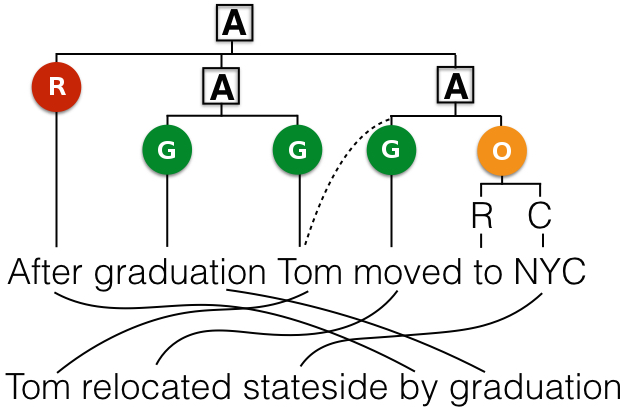
\includegraphics[width=0.35\textwidth]{ucca-tree-mteval-v2.png}
    \end{center}
  \caption{\label{fig:hume_tree_v2}
     HUME annotation of an UCCA tree with a word aligned example translation shown below. 
Atomic units are labelled using traffic lights (Red, Orange, Green) and structural units are marked A or B.}
\end{figure}
% Ondrej removes the following, he thinks that errors are not supposed to be
% propagated in HMEANT either:
%In HMEANT, it is not clear whether errors should be propegated up the SRL hierarchy. 

Figure~\ref{fig:hume_tree_v2} presents an example of a HUME
annotation, where the translation is in English for ease of comprehension.
When evaluating ``to NYC'' the annotator looks at the translation and sees the
word ``stateside''. This word captures the whole phrase and so we mark this
non-leaf node with an atomic label. Here we choose Orange since
it approximately captures the meaning in this context.
The ability to mark non-leaves with atomic labels allows
the annotator to account for translations which only correspond at the phrase
level. Another feature highlighted in this example is that by separating structural
and atomic units, we are able to define where an error occurs, and localise
the error to its point of origin. The linker ``After'' is translated incorrectly as ``by''
which changes the meaning of the entire sentence. This error is captured at
the atomic level, and it is labelled Red. The sentence still contains two scenes and
a linker and therefore we mark the root node as structurally correct, Adequate.

\begin{figure*}[t]
    \begin{center}
    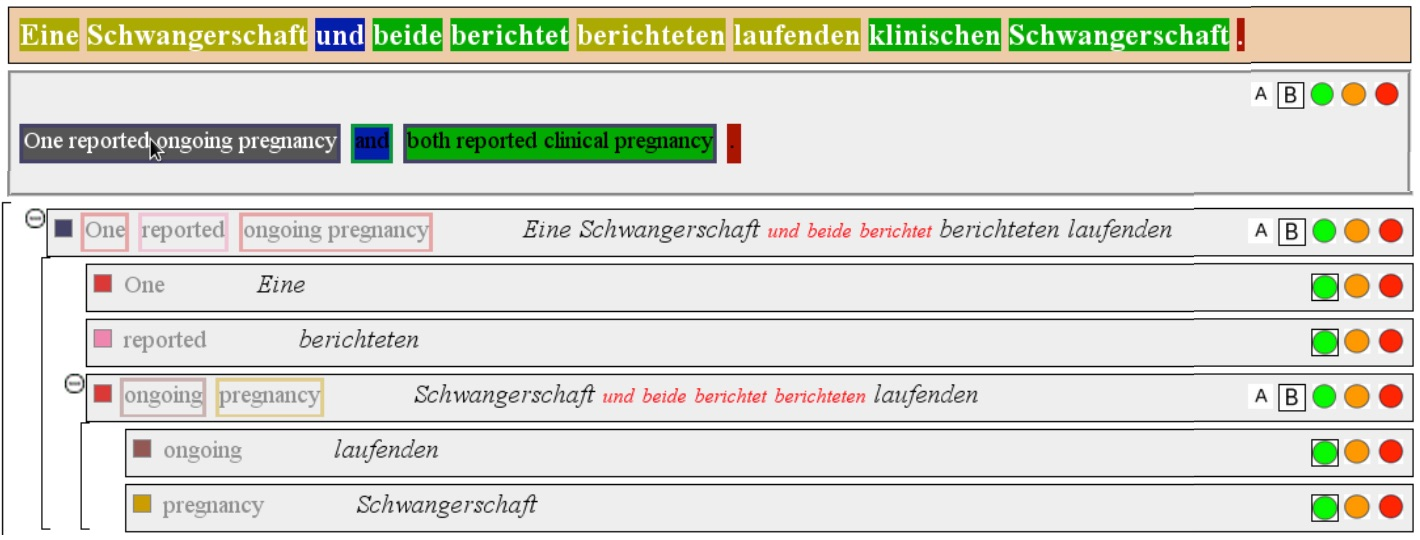
\includegraphics[width=.8\textwidth]{hume_interface2.jpg}
    \caption{The HUME annotation tool. The top orange box
      contains the translation. The source sentence is directly below it, followed by the tree of the source
      semantic units. Alignments between the source and translation are in italics and
      unaligned intervening words are in red (see text).}
    \label{fig:interface}
    \end{center}
\end{figure*}


\subsection{Composite Score}\label{sec:score}

We proceed to detailing how judgements on the semantic units
of the source are aggregated into a composite score. 
%While future extensive empirical evaluation with HUME and its application to MT
%system tuning may suggest more complex definition,
%as a starting point we take a parsimonious approach,
We start by taking a very simple approach and compute an accuracy score.
Let $\Green(s,t)$, $\Adequate(s,t)$ and $\Orange(s,t)$ be the number of Green, Adequate and Orange
units, respectively. Let $\Units(s)$ be the number of units marked with any of the labels.
Then HUME's composite score is:

\vspace{-.5cm}
{\scriptsize
\begin{equation}
  \HUME(s,t) = \frac{\Green(s,t) + \Adequate(s,t) + 0.5\cdot \Orange(s,t)}{\Units(s)}
  \nonumber
\end{equation}
}
\vspace{-.5cm}


%%%%%%%%%%%%%%%%%%%%%%%%%%%%%%%%%%%%%%%%%%%%%%%%%%%%%%%%%%%%%%%%%%%%%%%%%%
\subsection{Annotation Interface}

\figref{fig:interface} shows the HUME annotation interface.
% We now describe the HUME annotation interface, shown in \figref{fig:interface}. 
% %We turn to discuss the interface for collecting human judgements on the semantic units
% %of the source, relating to the translation. 
% UCCA annotations of the source are done offline,
% using the UCCA web application.
% %\figref{fig:interface} presents the user interface of HUME. 
% The translation appears at the top, and
% the source sentence directly below it. Underneath the source sentence appears
% its list of semantic units. 
% %For each semantic unit, including the one for the
% %entire source sentence, there is a textbox, displaying the yield of that unit.
% %Information on the category of the unit (e.g., whether it is a Scene, participant etc.).
The user is asked to select a label for each source semantic unit,
by clicking the ``A'', ``B'', Green, Orange, or Red buttons to the right of the unit's box.
Units with multiple parents (as with ``Tom'' in \figref{fig:hume_tree_v2}) are displayed
twice, once under each of their parents, but are only annotatable in one of
their instances, to avoid double counting.
%Note that the UCCA labels are not shown.

The interface presents, for each unit, the translation segment aligned with it.
This allows the user, especially in long sentences, to focus her attention on the parts
most likely to be relevant for her judgement. As the alignments are automatically derived,
and therefore noisy, the annotator is instructed to treat the aligned text is a cue, but to ignore
the alignment if it is misleading, and instead 
make a judgement according to the full translation.
Concretely, let $s$ be a source sentence, $t$ a translation,
and $A \subset 2^{s \times t}$ a many-to-many word alignment.
If $u$ is a semantic unit in $s$, whose yield is $yld(u)$, we define the aligned text in
$t$ to be $\bigcup_{(x_s,x_t) \in A \wedge x_s \cap yld(u) \neq \emptyset} x_t$.

Where the aligned text is discontinuous in $t$, words between the left
and right boundaries which are not contained in it (intervening words)
are presented in a smaller red font. 
Intervening words are likely to change the meaning of the translation
of $u$, and thus should be attended to when considering whether the translation
is correct or not. 

For example, 
%consider the sentence $s=$``We're driving back on Friday'' and the German
%translation t=``Am Freitag fahren wir zur\"uck'' (lit. ``on Friday driving we back'').
%``driving back'' will be aligned to ``fahren ... zur\"uck'',
%and ``wir'' will be marked as intervening word. Another example
in \figref{fig:interface}, ``ongoing pregnancy'' is translated to
``Schwangerschaft ... laufenden'' (lit. ``pregnancy ... ongoing''). This alone
seems acceptable but the interleaving words in red notify the annotator to check
the whole translation, in which the meaning of the expression is not preserved.
The annotator should thus mark this structural node as Bad.

%The interleaving 
%German words shown in red should not occur there, and the annotator should take this 
%into account and mark this structural node as ``B'', bad. 

% Ondrej did the following in a footnote in Section 3.1 Annotation Procedure
%\bh{Somewhere we could explain that we
%could do a similar annotation with monolinguals, although it entails aligning
%reference and MT output}

%There are cases where we cannot usefully compare individual words in the source to words in the target.
%We often need to compare translation at the phrase level. If this is the case, then we can 
% treat the structural node as a lexical unit, and mark it with the traffic light labels. This 
%means that none of the children of this node will be examined in order determine the semantic score
%for this sentence. 
%In Figure~\ref{ucca-tree-mteval}, we can see that the phrase ``became a passion'' has been labelled as a lexical
%node and it has been evaluated as ``Orange'', or partially correct, as the translation of this phrase ``loved'' 
%only partially capture the semantics of the source.


\com{
In Figure~\ref{mttool}, we show the MT evaluation tool. The sentence at the top shows the complete MT system output. Underneath the MT output is the  source sentence.  Underneath the source sentence we see its expandable semantic tree structure with both lexical and structural nodes. atomic nodes only have traffic light annotation, whereas a structural node would normally be labelled ``A'' or ``B'' but could also be labelled as a lexical node, in the case where there is no word to word correspondence for the translation of its children.

 The child components of a structural node are marked with different coloured rectangles. When navigating through the different source sentence nodes, one can see the relevant sections of the translation because the aligned words in the translation are highlighted in the complete sentence above. Aligned translations are also shown in black alongside the source node. If the node is aligned to a set of dis-contiguous words in the translation, then the unaligned words that appear in between the aligned words are shown in red. Even if these words are not directly aligned to the source node, they 
will likely change the meaning of the translation and must be considered when marking 
the translation as correct or not. The alignments are meant just as a guide. The annotator should  look at the complete translation when deciding on the evaluation of a node. The translation could have content added before or after the node which changes its
 structure or meaning. If an extra component is prepended to a structural node, for example, it should be marked as ``Bad''.
}

%%%%%%%%%%%%%%%%%%%%%%%%%%%%%%%%%%%%%%%%%%%%%%%%%%%%%%%%%%%%%%%%%%%%%%%%%%%%%%%%%%%
\section{Experiments}\label{sec:experiments}


In order to validate the HUME metric, we ran an annotation experiment with one source language (English),
and four target languages (Czech, German, Polish and Romanian), using text from the public health domain.
Semantically accurate translation is paramount in this domain, which makes
it particularly suitable for semantic  MT evaluation. HUME is both evalauted in terms of its
consistency (inter-annotator agreement), efficiency (time of annotation) and validity (through a comparison
with crowd-sourced adequacy judgements).

%particularly interested in this domain since our ultimate goal is to provide high-quality translations of health
%information for speakers of languages other than English, and in this domain accurate transfer of meaning is
%paramount.

%The experiment seeks to address two questions:
%\begin{inparaenum}
%\item Can HUME be annotated quickly and reliably, and does the reliability still hold for longer sentences?
%\item Can HUME capture translation issues that other annotation schemes (such as adequacy judgements
%  and HMEANT) cannot?
%\end{inparaenum}

%\item What can HUME annotation tell us about the strengths and weaknesses of MT?
%\bh{Maybe we should remove the third one, we
%probably don't address it in this paper}


\subsection{Datasets and Translation Systems}

For each of the four language pairs under consideration  we built phrase-based MT systems
using Moses \parcite{Koehn:2007}.  These were trained on large parallel data sets extracted from
OPUS \parcite{tiedemann:2009}, and the data sets released for the WMT14
medical translation task \parcite{bojar-EtAl:2014:W14-33}, 
giving between 45 and 85 million sentences of training data, depending on language pair.
%\oa{I think we should probably
%  say how many in each.}.
% ... if someone asks us to do so...
These translation systems were used to translate texts derived from both NHS
24\footnote{\url{http://www.nhs24.com/}} and
Cochrane\footnote{\url{http://www.cochrane.org/}} into the four languages.
NHS~24 is a public body providing healthcare and health-service
related information in Scotland, Cochrane is an international NGO
which provides independent systematic reviews on health-related research.
NHS~24 texts come from the ``Health A-Z'' section in the NHS Inform
website, and Cochrane texts come from their plain language summaries
and abstracts.

%\bh{How much more do we need? Perhaps in the intro we could justify our focus on public health text
%(accuracy!). The test corpora should have a public URL by the time we submit, although of course the source texts were 
%already public anyway, and Lexi did some selection of examples for use in this expt. -- do we have to explain this?}
% ... todo for the camera ready, if we get through

\subsection{HUME Annotation Statistics}
\label{sec:annot_stats}

The source sentences are all in English, and their UCCA annotation was performed by four
computational linguists and one linguist.
For the annotation of the MT output, we recruited two annotators for each of German, Romanian
and Polish and one main annotator for Czech. For Czech IAA,
several further annotators worked on a small number of 
sentences each. We treat these further annotators as one annotator, resulting in two annotators
for each language pair.
The annotators were all native speakers of the respective target languages and fluent in English.
\oa{maybe we should put in what training they've received}

\tabref{tab:annot}
shows the total number of sentences and units annotated by each annotator.
Not all units in all sentences were annotated, often due to
the annotator %not finishing a sentence or
accidentally missing a node.
%, but in many cases it was also because it was an implicit 
%UCCA node, which was not shown to the annotators since there is no corresponding source segment.
\begin{table}
\begin{center}
{\small
\begin{tabular}{ll|cccc}
& & cs & de & pl & ro \\
\hline
\#Sentences &  Annot. 1 & 324   & 339  & 351  & 230  \\
 & Annot. 2 & 205 & 104  & 340  & 337 \\
\hline
\#Units & Annot. 1 & 8794  & 9253 & 9557  & 6152 \\
 &Annot. 2 & 5553 & 2906  & 9303  & 9228  \\
\end{tabular}
\caption{HUME-annotated \#sentences and \#units.}
\label{tab:annot}
}
\end{center}
\end{table}

\paragraph{Efficiency.}
We estimate the annotation time using the timestamps
provided by the annotation tool, which are recorded whenever an annotated sentence is
submitted. Annotators are not able to re-open a sentence once submitted. 
To estimate the annotation time, we compute the time difference between successive 
sentences, and discard outlying times since we assume annotation was not continuous.
From inspection of histograms of annotation times, we set the upper threshold at 500 seconds.
Median annotation times are presented in Table~\ref{tab:annot_times},
indicating that the annotation
of a sentence takes around 2--4 minutes, with some variation between annotators.

%The annotators worked remotely at their own pace, so no precise timing information is available.
%Nevertheless

\begin{table}[t]
\begin{center}
{\small
\begin{tabular}{l|cccc}
& cs & de & pl & ro \\
\hline
Annot. 1 & 255 & 140  & 138 & 96 \\
Annot. 2 & $^*$ & 162 & 229 & 207 \\
\end{tabular}
\caption{Median annotation times per sentence, in seconds.
  $^*$: no timing information is available, as
  this was a collection of annotators, working in parallel.}
\label{tab:annot_times}
}
\end{center}
\end{table}


%\XXX{Describe the UCCA annotation}
% ... not enough room or time


\paragraph{Inter-Annotator Agreement.}
\label{sec:iaa}

\begin{table}[t]
\begin{center}
{\small
\begin{tabular}{l|cccc}
 & cs & de & pl & ro \\
\hline
Sentences & 181 & 102 & 334 & 217 \\
\hline
All units & 4686   & 2793   & 8384   & 5604  \\
Kappa & 0.64   & 0.61   & 0.58   & 0.69  \\
\hline
Atomic units & 2982 & 1724 & 5386 & 3570 \\
Kappa & 0.54 & 0.29 & 0.54 & 0.50 \\
\hline
Structural units & 1602 & 1040 & 2655 & 1989 \\
Kappa & 0.31 & 0.44 & 0.33 & 0.58 \\
\end{tabular}
\caption{IAA for the multiply-annotated units,
measured by Cohen's Kappa. }
\label{tab:iaa}
}
\end{center}
\end{table}

%\oa{what is the purpose of the BLEU binning? is it because low quality and high
%quality translations often diverge in their agreement scores?}

In order to assess the consistency of the annotation, we measure the Inter-Annotator
Agreement (IAA) using Cohen's Kappa on the multiply-annotated units.
%For German, Polish and Romanian we used two annotators, with a significant overlap
%between the sentences they annotated. For Czech we had the entire batch
%annotated by one main annotator and multiple secondary annotators, 
%each annotating a sub-part of the batch.
\tabref{tab:iaa} reports the number of units which have two annotations from
different annotators and the corresponding Kappas.
%
%In order to compute Kappa, we consider the annotation task as a classification task on 
%nodes, and compute agreement on nodes which have two annotations from different annotators.
We report the overall Kappa, as well as separate Kappas on atomic
units (annotated as Red, Orange or Green) and structural units (annotated
as Adequate or Bad).
As expected and confirmed by confusion matrices in \figref{fig:heatmap}, there
is generally little confusion between the two types of units.

%In general there should be little confusion between the two
%types of nodes, and in future work the separation between the nodes should be enforced
%by the tool.
%\oa{but there may be some disagreement in the margins on what nodes are atomic and
%  what are not}
%The Kappas are shown in \tabref{tab:iaa}.


\def\iaafig #1{\includegraphics[width=3.8cm]{iaa_heatmap_#1.png}}

\begin{figure}[t]
\renewcommand{\tabcolsep}{0pt}
\begin{tabular}{cc}


\subfloat[English-Czech]{
  \iaafig{cs}
}
&
\subfloat[English-German]{
  \iaafig{de}

}
\\

\subfloat[English-Polish]{
  \iaafig{pl}
  
}
&
\subfloat[English-Romanian]{
  \iaafig{ro}

}
\end{tabular}
\caption{Confusion matrices for each language pair.}
\label{fig:heatmap}
\end{figure}



%presents the variance of kappa with length in each bin covers
%a length range of 10. and we show .

\def\iaafig #1{\includegraphics[width=3.8cm]{iaa_length_#1.png}}

To assess HUME reliability for long sentences,
we binned the sentences according to length and measured Kappa on each of the
bins (\figref{fig:iaalength}).
%The Kappas for each bin is presented in 
%\figref{fig:iaalength}.
%Results show that there is
We see
no discernable reduction of IAA with sentence
length. Also, from \tabref{tab:iaa} the overall IAA
is quite similar for all languages, showing good agreement (0.6--0.7).
However, there are differences observed when we break down by node type.
In particular, we see a contrast  between
Czech and Polish, where the IAA is higher for atomic than for structural units, and German and Romanian,
where the reverse is true. We also observe low IAA (around 0.3) in the cases of
German atomic units, and Polish and Czech structural units.

\begin{figure}[t]
\renewcommand{\tabcolsep}{0pt}
\begin{tabular}{cc}


\subfloat[English-Czech]{
  \iaafig{cs}
}
&
\subfloat[English-German]{
  \iaafig{de}

}
\\

\subfloat[English-Polish]{
  \iaafig{pl}
  
}
&
\subfloat[English-Romanian]{
  \iaafig{ro}

}
\end{tabular}
%\caption{Kappa versus sentence length, separately for
%structural and atomic units. The numbers are the node counts in each bin. }
\caption{Kappa versus sentence length for
structural and atomic units. (Node counts in bins on top of each bar.)
}
\label{fig:iaalength}
\end{figure}


Looking more closely at the areas of disagreement, we see that for the Polish structural units, the 
proportion of As was quite different between the two annotators (53\% vs. 71\%), whereas for other
languages the annotators agree in the proportions. We believe that this was because one of the Polish
annotators did not fully understand the guidelines for structural units, and percolated
errors up the tree, creating more Bs. For German atomic and Czech structural units, where Kappa is also around 0.3, the proportion of such units being marked as ``correct'' is relatively 
high, meaning that the class distribution is more skewed, so the expected agreement used in the
Kappa calculation is high, lowering Kappa.
%ssentially, the annotation problem is harder when the classes are more skewed.
Finally we note some evidence of domain-specific disagreements, for instance
the German MT system normally translated ``review'' (as in ``systematic review'' -- a frequent term in the 
Cochrane texts) as ``\"uberpr\"ufung'', which 
one annotator marked correct, and the other (a Cochrane employee) as incorrect.


\subsection{Comparison with Direct Assessment}\label{sec:adequacy}

\def\iaafig #1{\includegraphics[width=0.45\textwidth]{humevsDA_10en-#1.pdf}}

\begin{figure}[t]
\renewcommand{\tabcolsep}{0pt}
\begin{tabular}{c}
\subfloat[English-German]{
  \iaafig{de}
}
\\
\subfloat[English-Romanian]{
  \iaafig{ro}
}
\end{tabular}
\caption{HUME vs DA scores. DA score have been standardised for each crowdsourcing annotator and averaged across exactly 10 annotators. HUME scores are averaged where there were two annotations. 
%The regression is calculated using linear least squares.
}
\label{fig:dacorrelation}
\end{figure}

Recent research~\cite{graham2015accurate,graham2015crowd,graham2015improving} has proposed a new approach for collecting accuracy ratings, direct assessment (DA).
%By crowdsourcing a large number of adequacy judgements for each candidate translation on a fine-grained scale of 0 to 100, we can apply statistical measures which result in reliable aggregate scores, that correlate very strongly with one other.
Statistical interpretation of a large number of crowd-sourced adequacy
judgements for each candidate translation on a fine-grained scale of 0 to 100
results in reliable aggregate scores, that correlate very strongly with one
another.

We attempted to follow \perscite{graham2015accurate} but struggled to get enough
crowd-sourced judgements for our target languages. We ended up with 10 adequacy 
judgements on most of the HUME annotated translations for
German and Romanian but insufficient data for Czech and Polish. We see this as a
severe practical limitation of DA.
%We followed~\parcite{graham2015accurate} and collected 10 adequacy
%judgements on most of the HUME annotated translations for
%German and Romanian, using the CrowdFlower platform\footnote{\url{https://www.crowdflower.com}}. To ensure high quality judgments we restricted the IP of the annotators to those of the relevant country. Czech and Polish judgements were
%excluded, as our experiments only yielded very little high quality data.

Figure~\ref{fig:dacorrelation} plots the HUME score for each sentence against
its DA score. HUME and Direct Assesment scores correlate reasonably well. The
Pearson correlation for en-ro (en-de) is 0.70 (0.58), or 0.78 (0.74) if only
doubly HUME-annotated points are considered.
This confirms that HUME is consistent with an accepted human evaluation method,
despite the differences in their conception.
While DA is a valuable tool, HUME has two advantages:
it returns fine-grained semantic information about 
the quality of translations and it only requires very few annotators.
Direct assesment returns a single opaque score, and (as also noted by
Graham et al.), and requires a large crowd which may not be available or reliable. 

\begin{figure}[t]
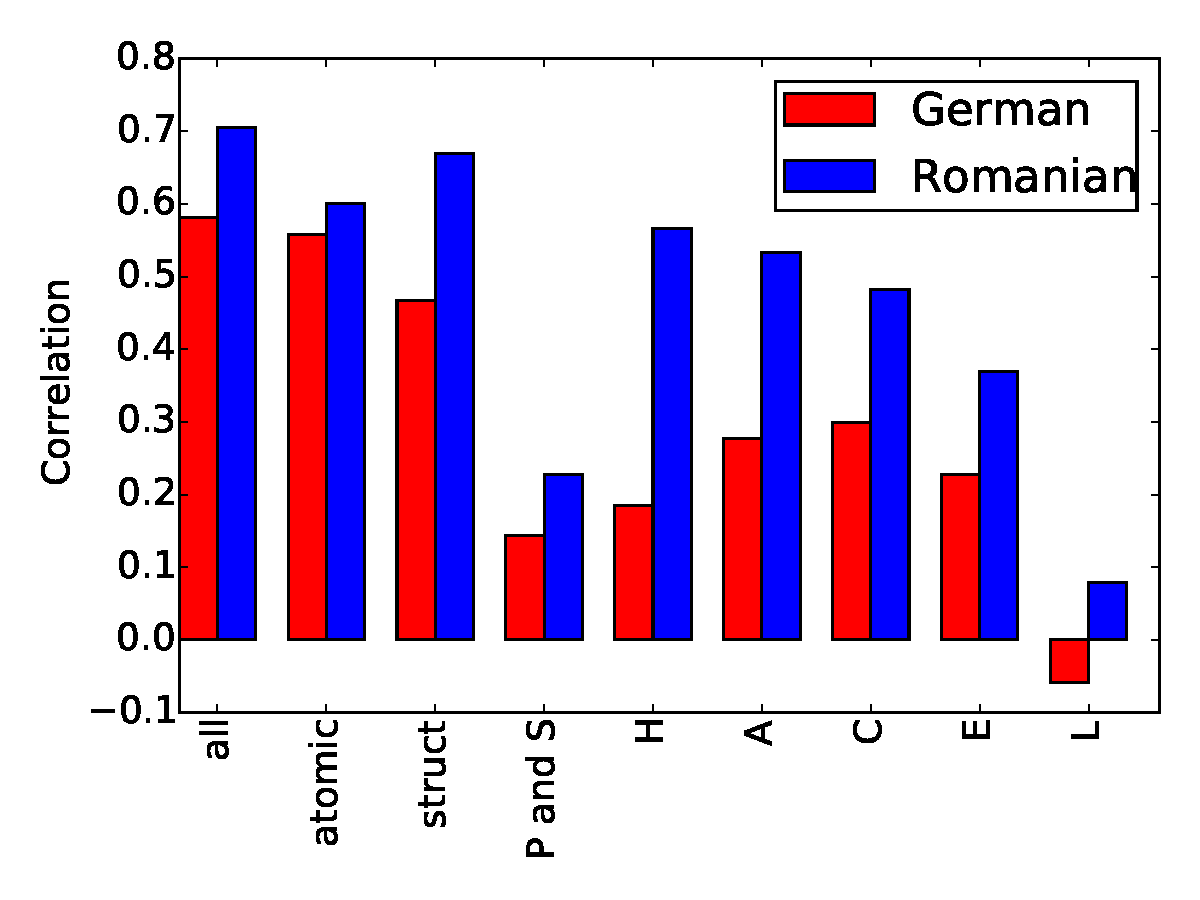
\includegraphics[width=0.45\textwidth]{humevsDAcorrtypes-10en-dero.pdf}
\caption{Pearson correlation of HUME vs. DA scores for different node types for both
  the en-de and en-ro experiments. See text for the bar legend.
%Struct refers to all structural nodes, P+S are all process and state nodes, H parallel scene nodes, A participant, C centre, E elaborators, and L linker nodes.}
\label{fig:dacorrelationtypes}}
\end{figure}


Figure~\ref{fig:dacorrelationtypes} presents an analysis of HUME's correlations with DA by HUME unit type,
an analysis enabled by HUME's semantic decomposition. 
Each bar represents a correlation between HUME and an aggregate HUME score
based on a sub-set of the units (\#nodes for the en-de/en-ro setting in brackets):
all units ('all', 8624/10885), atomic ('atomic', 5417/6888) and structural units ('struct', 3207/3997),
and units by UCCA categories: Scene main relations (i.e, Process and State units; 'P and S', 954/1178), Parallel Scenes ('H', 656/784),
Participants ('A', 1348/1746),
Centres ('C', 1904/2474), elaborators ('E', 1608/2031) and linkers ('L', 261/315).
In both settings correlation is highest in the 'all' case, supporting our claim for the value of aggregating over a wide range of semantic phenomena. Some types of nodes predict the DA scores better than others. HUME scores on As correlate more strongly with DA than scores on Scene Main Relations (P+S). Center nodes (C) are also more correlated than elaborator nodes (E), which is expected given that Centers are defined to be more semantically dominant. Future work will construct an aggregate HUME score which weights the different node types according to their semantic relevance. 


%\subsection{Discussion of Disagreements}\label{sec:disagreements}



%%%%%%%%%%%%%%%%%%%%%%%%%%%%%%%%%%%%%%%%%%%%%%%%%%%%%%%%%%%%%%%%%%%%%%%%%%%%%%%%%%%
\section{Comparison with HMEANT}\label{sec:hmeant_comp}

We discuss the main differences between HUME and HMEANT,
a human MT evaluation metric that measures the overlap between the translation a reference
in terms of their SRL annotations.

%Like HMEANT, HUME defines  a
%measure that decomposes over semantic units, rather than strings. 
%However, there are important differences in design decisions, which we summarize in this
%section.

\paragraph{Verbal Structures Only?}

HMEANT focuses on verbal argument structures, ignoring other pervasive phenomena such as non-verbal predicates and inter-clause relations. Consider the following example:

\vspace{-.3em}
\begin{center}
\begin{tabular}{lp{5.4cm}}
Source & \small a coronary angioplasty may not be technically possible \\
Transl.& \small eine koronare Angioplastie kann nicht technisch m{\"o}glich \\
Gloss & \small a coronary angioplasty can not technically possible \\
\end{tabular}
\end{center}
\vspace{-.5em}

%``a coronary angioplasty may not be technically possible'', which was translated by our en-de system
%to ``eine koronare Angioplastie kann nicht technisch m{\"o}glich'' (gloss: 
%a coronary angioplasty can not technically possible).

The German translation 
is largely correct, except that the main verb ``sein'' (``be'') is omitted.
While this may be interpreted as a minor error, HMEANT will assign the
sentence a very low score, as it failed to translate the main verb.
%
Conversely, HMEANT does not penalize errors such as tense or negation
flip in a correctly aligned predicate.

%This focus on verbal predicates has a number of unfortunate consequences. We show an example below:

% \noindent
% \begin{inparadesc}
% \item[Source ] a coronary angioplasty may not be technically possible \\
% \item[Transl.] eine koronare Angioplastie kann nicht technisch m{\"o}glich \\
% \item[Gloss ]  a coronary angioplasty can not technically possible \\
% \end{inparadesc}

\com{
}

We conducted an analysis of the English UCCA Wikipedia corpus (5324 sentences) in order to assess the pervasiveness of three phenomena that are not well supported by HMEANT.\footnote{Argument structures and linkers are explicitly marked in UCCA. Non-auxiliary instances of ``be'' and nouns are identified using the NLTK standard tagger. Nominal argument structures are here Scenes whose main relation is headed by a noun.}
First, copula clauses are treated in HMEANT simply as instances of the main verb ``be'', which generally does not convey the meaning of these clauses. They appear in 21.7\% of the sentences, according to conservative estimates that only consider non-auxiliary
instances of ``be''.
Second, nominal argument structures, ignored by HMEANT, are in fact highly
pervasive, appearing in 48.7\% of the sentences.
Third, linkers that express inter-relations between
clauses (mainly discourse markers and conjunctions) appear in 56\% of the
sentences, but are again ignored by HMEANT. As noted in our experiments, linkers
are sometimes omitted in translation, but these omissions are not taken
into consideration by HMEANT.

%An example where a linker is omitted in translation in our experiments is
%\equo{However, this review\dots}, which was translated to
%the German \equo{Diese \"Uberpr\"ufung\dots} (lit. \equo{This review}).
%This omission will not be taken into account by HMEANT at all

We are not aware of any empirical argument suggesting that verb argument structures,
taken alone, capture the crux of the sentence semantics.
Moreover, relying only on verbal argument structures is less stable across paraphrases
and translations, as a verbal argument structure
may be translated to a nominal or adjectival argument structure
(e.g., ``after graduation'' may be translated into ``after he graduated'').
This may lead to an unduly low HMEANT score, as the verb
in one structure has nothing to align to in the other.
On the other hand, UCCA has been shown to be reasonably stable in an English-French
corpus study \cite{sulem2015conceptual}.

% No space
%It is also relatively common in translation that verbal constructions get
%nominalized or vice versa. An example from our dataset:
%  ``Two {\bf review} authors assessed the studies independently\dots{}'' --
%  ``Zwei Autoren bewertete die Studien unabh\"angig zu {\bf
%  \"uberpr\"ufen}\dots{}'' (lit. ``Two authors assessed the studies
%  independently to review\dots").\XXX{This is Omri's example, with
%  Ondrej's gloss for German. Ondrej is
%  not totally sure that the meaning is well preserved. So Ondrej would actually
%  *remove* this example, because it would illustrate HMEANT's problems only if
%  the meaning was correct.}

We note that some of these issues were already observed
in previous applications of HMEANT to languages other than
English. See \perscite{birch-EtAl:2013:WMT} for German, \perscite{bojar:wu:ssst:2012} for
Czech and \perscite{chuchunkov-tarelkin-galinskaya:2014:SSST-8} for Russian.




% I am not sure that this is true
%The coverage of
%these and other phenomena by HUME will allow to empirically determine 
%(rather than stipulate), which semantic structures are important
%to preserve for MT evaluation, and which are less important.

%
%\paragraph{Cost of Structural Annotation}
%
%HMEANT structural annotation (semantic role labelling, SRL), similar to e.g.
%PropBank
%\parcite{palmer2010semantic}, is designed to be very simple and easy to explain
%to lay annotators.
%HUME relies on UCCA, which is arguably more abstract, harder to
%explain, and thus more expensive to obtain.
%
%On the other hand, HUME 
%needs the semantic annotation
%done once for a given source sentence, whereas for the HMEANT set-up, every new
%MT output has to be structurally annotated.\oa{we can give some empirical data here.

%\oa{we can give some empirical data here.
%  In the WMT 13 experiment, Lexi and Barry report a little over 3 mins of annotation
%  per sentence + 3 translations. HUME annotation is about 2-4 minutes per sentence.
%  UCCA annotation by trained annotators is about 700 tokens/hour (we didn't
%  check it for individual sentences), but that's done only once so it should be amortized.}

\paragraph{One Structure or Two.}
HUME only annotates the source, while HMEANT relies on
two independently constructed structural annotations, one for the reference and one
for the translation.
%First of all, the annotation process is different. We semantically annotate the
%source, then automatically project it to the translation, and ask bilingual
%annotators to assess whether this projection shows a good or bad translation. In
%HMEANT, they semantically annotate both the reference and the translation, then
%align these manually, and assess to what extent they match.
%We see this difference as crucial where semantic analysis is concerned, as it
Not annotating the translation is appealing as it is often impossible to assign a
semantic structure to a low quality translation.
On the other hand, HUME may be artificially boosting the perceived understandability
of the translation by allowing access to the source.


\paragraph{Alignment.}
In HMEANT, the alignment between the reference and translation structures is a key
part of the manual annotation. If the alignment cannot be created, the 
translation is heavily penalized.
\perscite{bojar:wu:ssst:2012} and \perscite{chuchunkov-tarelkin-galinskaya:2014:SSST-8}
argue that the structures of the reference and of an accurate translation
may still diverge, for instance due to a different
interpretation of a PP-attachment, or the verb having an additional modifier in
%suggested that sometimes, the structures of the reference and candidate
%translations diverge without any good reason, for instance due to a different
%interpretation of a PP-attachment, the verb can have one additional modifier in
one of the structures. It would be desirable to allow modifications to
the SRL annotations at the alignment stage,
to avoid unduly penalizing such spurious divergences.
%annotations also at the alignment stage
%to avoid unduly penalization due to such a spurious divergence.
The same issue is noted by \perscite{lo:wu:reliability:2014}:
the IAA on SRL dropped from 90\% to 61\% 
when the two aligned structures were from two different annotators.
HUME uses automatic (word-level) alignment, which only
serves as a cue for directing the attention of the annotators.
The user is expected to mentally correct the
alignment as needed, thus circumventing this difficulty.


%HUME uses only automatic (word-level) alignment, which only serves as a cue for directing
%the attention of the annotators.
%The user is expected to mentally correct the alignment as needed.



\paragraph{Monolingual vs. Bilingual Evaluation.}
\label{src-vs-ref}
HUME diverges from HMEANT and from shallower measures
like BLEU, in not requiring a reference.
Instead, it compares the source directly with the output translation.
This requires the employment of bilingual annotators, but has the benefit of avoiding
using a reference, which is never uniquely defined, and may thus 
lead to unjustly low scores where the translation is a paraphrase of the reference.

%If only monolingual annotators are available, the HUME evaluation could be performed
%with a reference sentence instead of with the source. 
%\bh{But this would be a different metric}

% While HUME avoids this problem,
%imposing a structure only on the source does prevent any fine-grained semantic
%analysis of the translation.

%Perhaps more importantly, references are often not created by translating the source
%sentences. In some cases, the manual translation was actually carried out in the
%other direction, from ``reference'' to ``source''
%and in others the ``source'' and ``reference'' are independent translations
%from a third language. ``References'' can thus easily contain information
%that does not appear in the ``source''.

\com{
\paragraph{Error Localisation.}
In HMEANT, an error in a child node often results in the parent node
being penalised as well. This makes it harder to quantify the true scale of  
the original error, as its effect gets propagated up the tree. 
In HUME, errors are localised as much as possible to where they occur,
by the separation of atomic and structural units,
which supports a more accurate aggregation of the translation errors
to a composite score.
}
%\oa{Omitted point here} % OB: Added a sentence covering it: Conversely,
%HMEANT does not...

%I see this a falling under the verbal structures point
%\paragraph{Annotation of Predicates Themselves}

%HUME allows to annotate multi-word and even
%non-contiguous elements as a single unit. HMEANT, on the other hand, always
%required exactly one word to be annotated as the predicate, which
%is often linguistically inadequate.

%Another problem with HMEANT identified by \perscite{bojar:wu:ssst:2012} was the
%inability to indicate that the predicate is somewhat mistranslated (e.g.
%accidentally negated or in a slightly wrong tense). HMEANT
%annotation allows either to mark the source and reference frames as matching
%(which implies that the corresponding predicates are correct translations of each
%other), or as non-matching (which leads to a zero score for the whole frame) but
%nothing in between. In HUME, the verb is still present as a sub-unit of the
%frame and has the traffic-lights annotation.

  
% \Subsectionngigngig zu  Zu { to be removed}
% 
% In the *MEANT papers they mainly test by either
% A) correlating the metric to ranking judgements; or
% B) using automated versions of the metric for tuning MT systems
% 
% I think neither is particularly convincing, but I'm not sure at the moment what we replace them with. Dekai also made a claim about the *MEANT metrics being "interpretable" in the sense that they could guide you towards semantic errors that the MT system may be making, however I don't recall seeing this done in his papers. 
% 
% By the claim that HMEANT explains things, Dekai probably means that the score is decomposable, but so is UCCA-Eval and even BLEU. And UCCA-Eval has one benefit over HMEANT: it points to words in the MT output that are aligned with something but do not convey the meaning well (and we know which part of the source meaning). Pure HMEANT might say only that some part of the MT output has no clear frames whatsover (and we do not know which part of the source/reference, unless we add the word alignments).
% 
% 



%Here is an additional argument to support the need for target-only intelligibility:
%http://www.aclweb.org/anthology/W14-4005
%see Table  3 and the text in Section 5.2.
%The more frames can people annotate in the hypothesis, the better the hypothesis overall.







%%%%%%%%%%%%%%%%%%%%%%%%%%%%%%%%%%%%%%%%%%%%%%%%%%%%%%%%%%%%%%%%%%%%%%%%%%%%%%%%%%%
\section{Conclusion}\label{sec:conclusion}

We have introduced HUME, a human semantic MT evaluation measure which addresses
a wide range of semantic phenomena. We have shown that it can be reliably and 
efficiently annotated in multiple languages,
and that annotation quality is robust to sentence length.
We believe that
HUME, and a future automated version of HUME, allows for a more fine-grained analysis of translation quality,
and will be to guide the development of a more semantically aware approach to MT.






%%%%%%%%%%%%%%%%%%%%%%%%%%%%%%%%%%%%%%%%%%%%%%%%%%%%%%%%%%%%%%%%%%%%%%%%%%%%%%%%%%%
\com{
\section{Human Semantic Evaluation}

\oa{mention TER: using insertions, deletions, substitutions and shift of the entire sentence}

\label{sec:sem-eval:human}
We focus on producing high accuracy machine translation systems, but common 
automatic MT metrics are not able to directly capture accuracy. Even previously suggested methods
for using humans to evaluate accuracy are highly problematic. We aim to  develop a human evaluation method 
which is reliable and affordable and apply it to the MT prototypes. 
%This 
The
work described
in this section relates to 
%the 
task
\emph{T5.2: Human semantic evaluation}.
% defined in the description of action. 


In November 2015, we ran an evaluation task with 6 bilingual annotators, 2 from NHS 24 and 4 from Cochrane. 
We asked them to annotate about 350 sentences translated with the HimL year one systems 
and they had a budget of  up  to 40 hours each to perform this task. 
In this section we motivate and describe the experiment that we ran and we provide an initial analysis of
the results. In  Year 2 and Year 3 we will refine this evaluation task and use it to track the progress of our HimL prototypes.


\subsection{Overview}

Semantic evaluation of machine translation has typically been done at the sentence level and
we propose an  approach which breaks down the evaluation into basic semantic units, making evaluation 
simpler and more consistent. 
Our  assumption is that the semantic structure on the source sentence should be 
retained in the translation, and if it is not, then some essential part of the meaning 
%will be 
is
lost. 
The semantic framework that we base our evaluations on is called 
Universal Conceptual Cognitive Annotation \shortcite{abend2013universal}.  
UCCA has been developed using linguistic theories about 
what types of components and structures are universal across many different languages.

Our goal is to quantify how much of the meaning of the source sentence is preserved through translation.
There have been many approaches to evaluating the quality of machine translation, but most of them
have asked the annotator to give a score for the entire sentence. There are of course many ways 
that a translation can be incorrect and asking an annotator to provide a global score for a sentence
is a cognitively difficult task even if e.g. limited to a relative comparison
with another candidate translation. How serious is an error? What is the impact of multiple errors on global meaning?
By using UCCA structure to break the evaluation into meaningful components, we provide 
a more consistent and reliable method of evaluating translation accuracy.

The annotation proceeds as follows. Firstly, the source sentences (English, in our case) are annotated with UCCA trees. This
annotation is normally performed by computational linguists, and requires some training in UCCA, but the annotation can be 
reused for different target languages and different MT systems. 
We then create translations of the source sentences with the
MT system, collecting the word alignments from 
%
the
source sentence to 
the
translation provided by the system. These word
alignments are used to project the UCCA annotation from the source sentence to the the translation output, and then bilingual
annotators go through each projected UCCA node, assessing how well it is translated.  
We can estimate the impact of individual errors given their location in the semantic structure 
and we can thus extract a score for the whole sentence. More details on the procedure are provided 
below.


\subsection{Semantic Annotation}

The source sentences in this annotation scheme have been annotated with  a semantic structure defined as
Universal Conceptual Cognitive Annotation (UCCA).  UCCA was developed in the Computational Linguistics Lab of the Computer Science Department of the Hebrew University by Omri Abend and Ari Rappoport.
UCCA views the text as a collection of scenes (or events)
and their inter-relations and participants. 

\begin{figure*}[t]
    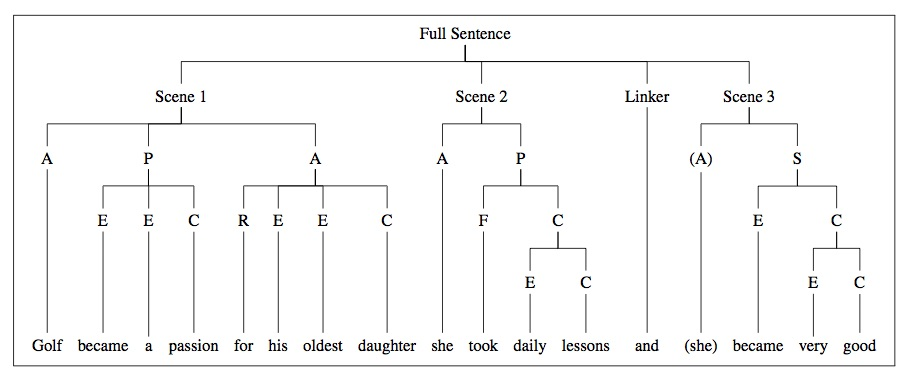
\includegraphics[width=1\textwidth]{ucca-tree.jpg}
    \caption{UCCA Tree with scenes}
    \label{ucca-tree}
\end{figure*}

%As you can see 
As can be seen
in Figure~\ref{ucca-tree}, the UCCA annotation results in a tree structure where each leaf is linked to
a word in the sentence at the bottom. A scene must contain a process (P) or a state (S). It can also contain
participants (A) and it can be linked to other scenes by a linker (Linker). Participants, processes and states can be
further analysed into elaborators (E), centres (C) and relators (R). These labels are very 
%high level 
high-level 
and relate to
cognitive concepts which should remain stable across languages.  

The fact that in UCCA
the labels are cognitive concepts and that they are linked directly to words
are both advantages 
when considering which semantic formalism is appropriate for machine translation evaluation.

One of such alternative formalisms is
Abstract Meaning Representation 
%%% Macro broken?
%(AMR; \inparcite{banarescu2013amr}). 
\parcite{banarescu2013amr}. 
AMR is being actively developed with 
%the view to 
a view towards
using it as a way of generating 
translations but AMR graphs are not aligned to the words in the sentences. Having more abstract semantic structures 
makes the link between source words, target words, and structures more complex and potentially less useful. 
Furthermore, AMR  has been developed mainly with English in mind, and it remains
to be seen how universal AMR graphs are. See
\shortcite{amr:interlingua:lrec:2014} for first observations of divergences
between English 
%vs.
vs.\ 
Chinese and
Czech AMRs.

Another possible semantic framework for this kind of MT evaluation is Semantic
Role Labelling 
%(SRL; \inparcite{palmer2010semantic}).
\parcite{palmer2010semantic}.
SRL has been used in a human translation metric called HMEANT~\parcite{lo2011structured}. 
HMEANT uses semantic role labels
to measure how much of the “who, why, when,
where” has been preserved in translation. Annotators are instructed to identify verbs as
heads of semantic frames. Then they attach role
fillers to the heads and finally they align heads
and role fillers in the candidate translation with
those in a reference translation. Using SRL for evaluating SMT has a number of
disadvantages as explored by
\shortcite{birch-EtAl:2013:WMT} for German, \shortcite{bojar:wu:ssst:2012} for
Czech and by \shortcite{chuchunkov-tarelkin-galinskaya:2014:SSST-8} for Russian.
The most important drawbacks are as follows:
\begin{itemize}
\item SRL frames are based around a verb which is particularly problematic for
copular verbs and  when verbs are translated correctly as nouns or correctly
omitted (the verb ``to be'' in some Russian constructions).
\item SRL frames do not cover the entire source sentence and the semantic structure is
therefore not completely defined, importantly links between frames are not
considered and prepositional phrases which attach to nouns are not marked.
\item Even considering a limited set of eleven roles (agent, patient,
experiencer, locative etc.) is problematic because we cannot assume that these roles will 
 remain stable across different languages. 
 When looking at an automatically parsed  English-Chinese  parallel corpora,
 it was shown that 8.7\% of the arguments do not preserve their semantic
 roles~\parcite{fung2006automatic}. 
\end{itemize}

UCCA provides universal semantic structures which 
%has 
have
a minimal set of labels. It provides a complete semantic tree which does not rely on syntactic heads and the semantic structure is grounded directly to the words in the sentence. 
 Even though the set of UCCA labels are fairly restricted,  nevertheless they allow us to determine the most important components of the graph (for example it defines centres and linkers which would be likely to carry more weight than elaborators), and we can use this to better calculate the score. 
We think that UCCA is the
most promising representation for evaluating translation. 
}

%\section*{Acknowledgments}

%Do not number the acknowledgment section.
%This section should not be presented for the submission version.

\bibliography{main}
\bibliographystyle{emnlp2016}


\end{document}
